%% Esempio per lo stile supsi
\documentclass[twoside]{supsistudent} 
\usepackage{graphicx}
\usepackage{subcaption}
\usepackage{hyperref}

% per settare noindent
\setlength{\parindent}{0pt}


% Crea un capitolo senza numerazione che pero` appare nell'indice %
\newcommand{\problemchapter}[1]{%
  \chapter*{#1}%
  \addcontentsline{toc}{chapter}{#1}%
\markboth{#1}{#1}
}

% Numerazione delle appendici secondo norma
\addto\appendix{
\renewcommand{\thesection}{\Alph{chapter}.\arabic{section}}
\renewcommand{\thesubsection}{\thesection.\arabic{subsection}}}

\setcounter{secnumdepth}{5} 	%per avere più livelli nei titoli
\setcounter{tocdepth}{5}		%per avere più livelli nell'indice


\titolo{DocTT --- Document Tagging Tool}
\studente{Cristian Spozio \vspace{1em}\\Denys Vitali}
\relatore{Daniele Puccinelli}
\correlatore{Salvatore Vanini}
\corso{Ingegeneria Informatica}
\modulo{M02042 - Progetto di semestre}
\anno{2019}



\begin{document}

\pagenumbering{alph}
\maketitle
\onehalfspacing
\frontmatter


\pagenumbering{roman}
\tableofcontents
\listoffigures					% Opzionale
\listoftables					% Opzionale

\newpage
\mainmatter
\pagenumbering{arabic}
\setcounter{page}{1}

\chapter*{Abstract}
\textit{DocTT} (Document Tagging Tool) is a tagging tool (corpus annotation tool)
which allows its users to tag text documents such as press conferences,
conference calls or pitches.
DocTT satisfies the need to switch from outdated tools such as 
\href{http://www.corpustool.com/}{UAM Corpus Tool} in order to provide an easy, open source,
multi-platform, lightweight and customizable tool to replace these outdated tools. \\
The tags take form in coloured rectangles
surrounding the text allowing a fast and easy visual recognition of a tag.
Tags are defined through a pre-uploaded tree by the user. The files involved
(document files and tree files) follow the XML standard and their parsing is 
managed by the tool.

\chapter*{Riassunto}
\textit{DocTT} è uno strumento di tagging di corpus testuale che utilizzato per
suddividere parti di testo ed assegnare delle etichette a parti di discorsi.
Il suo impiego principale è il tagging di conference calls, pithces o documenti
testuali in generale.

DocTT soddisfa il bisogno di cambiamento "imposto" da tool come 
\href{http://www.corpustool.com/}{UAM Corpus Tool} e fornisce 
un'alternativa open source multi-piattaforma, leggera e personalizzabile
per rimpiazzare questi strumenti. \\
\\
I tag sono rappresentati da rettangoli arrotondati e colorati che
circondano il testo, in modo da fornire un veloce riconoscimento di parti del
discorso. I tag sono definiti mediante un'albero caricato precedentemente
dall'utente. I file utilizzati (file di documento e dell'albero) seguono
lo standard XML e le convenzioni di UAM Corpus Tool. La loro interpretazione
è gestita dal nostro strumento.

\chapter{Introduzione}

\section{Struttura}

\textit{DocTT} si divide in 4 sezioni ognuna adibita ad una funzione specifica:
\begin{itemize}
  \item Home
  \item Document Upload
  \item Tree View
  \item Tree Upload
\end{itemize}

\subsection{Home}
La \textbf{Home} di \textit{DocTT} è la sezione in cui viene presentata la 
lista dei documenti caricati, dalla quale è possibile accedere ai documenti 
singoli e quindi alla loro modifica.

\begin{figure}[h!]
  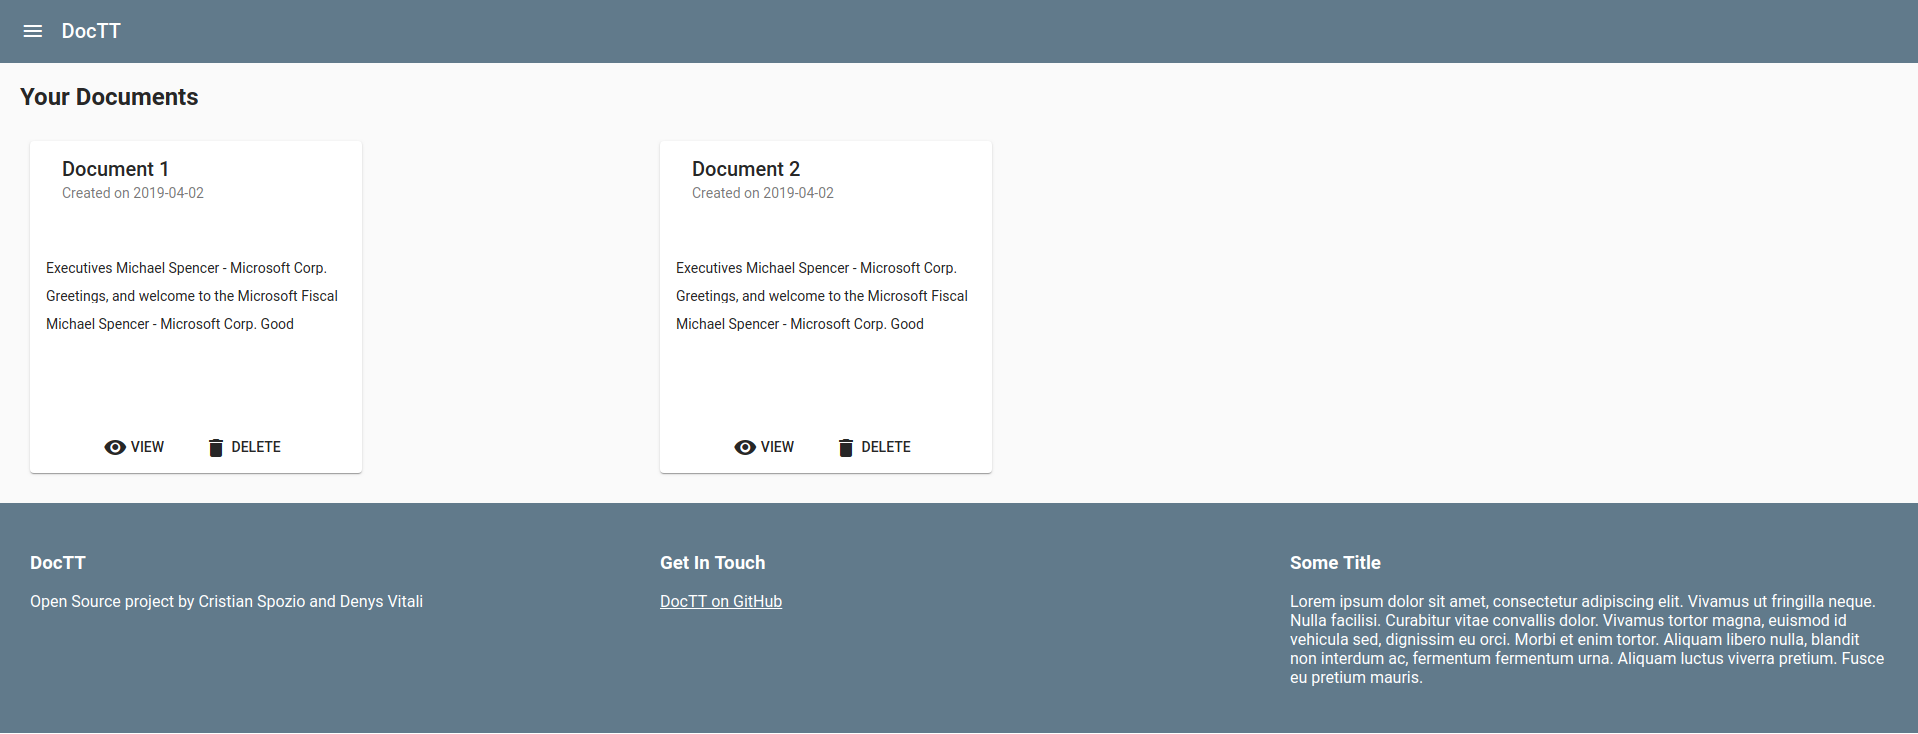
\includegraphics[width=\linewidth]{figures/home.png}
  \caption{Home section}
  \label{fig:home}
\end{figure}

\pagebreak

\subsection{Document Upload}
La sezione \textbf{Document Upload} di \textit{DocTT} è quella che permette
l'upload dei documenti da taggare ed il loro salvataggio nello storage del 
browser.

\begin{figure}[h!]
  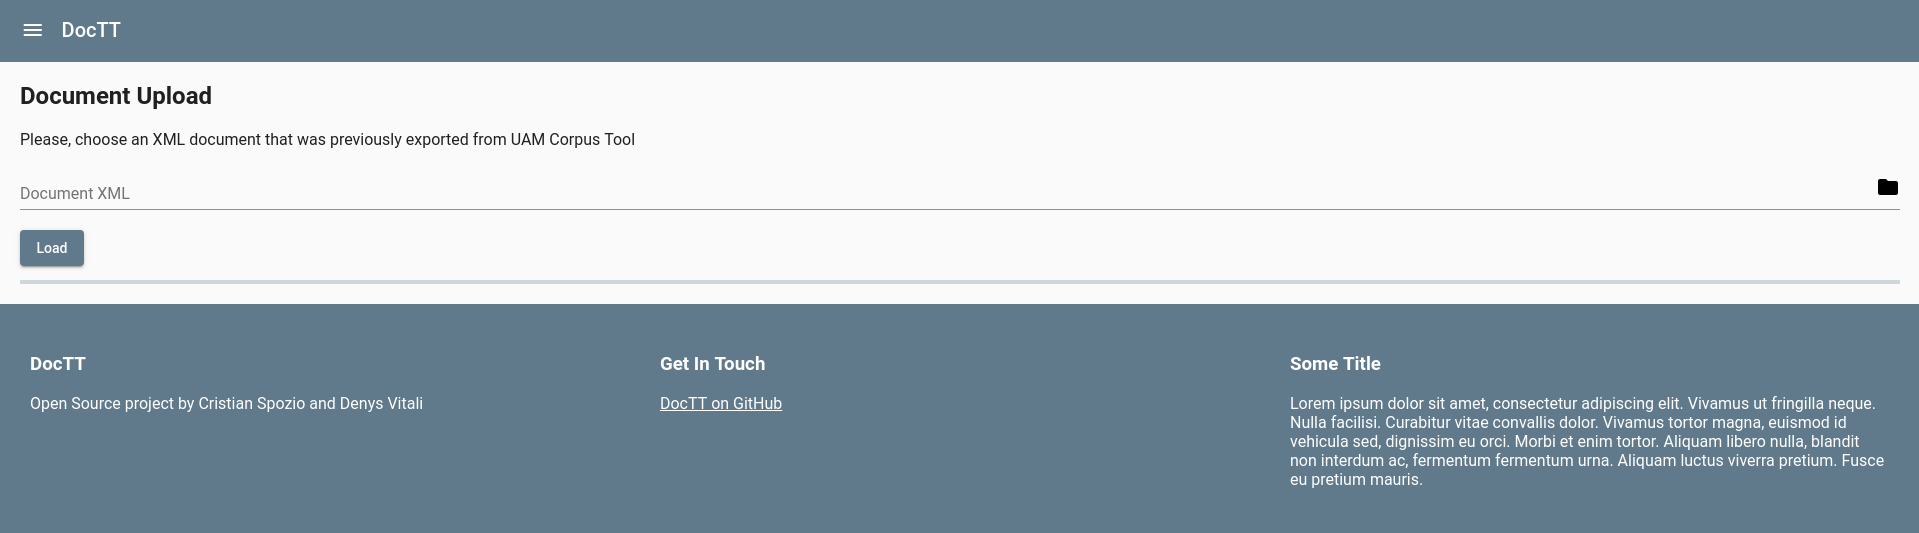
\includegraphics[width=\linewidth]{figures/docUpload.png}
  \caption{Document Upload section}
  \label{fig:docUpload}
\end{figure}

\subsection{Tree View}
La sezione \textbf{Tree View} di \textit{DocTT} è la parte che mostra l'albero
di tagging attualmente in uso come un elenco puntato espandibile per ogni
sottosezione presente.

\begin{figure}[h!]
  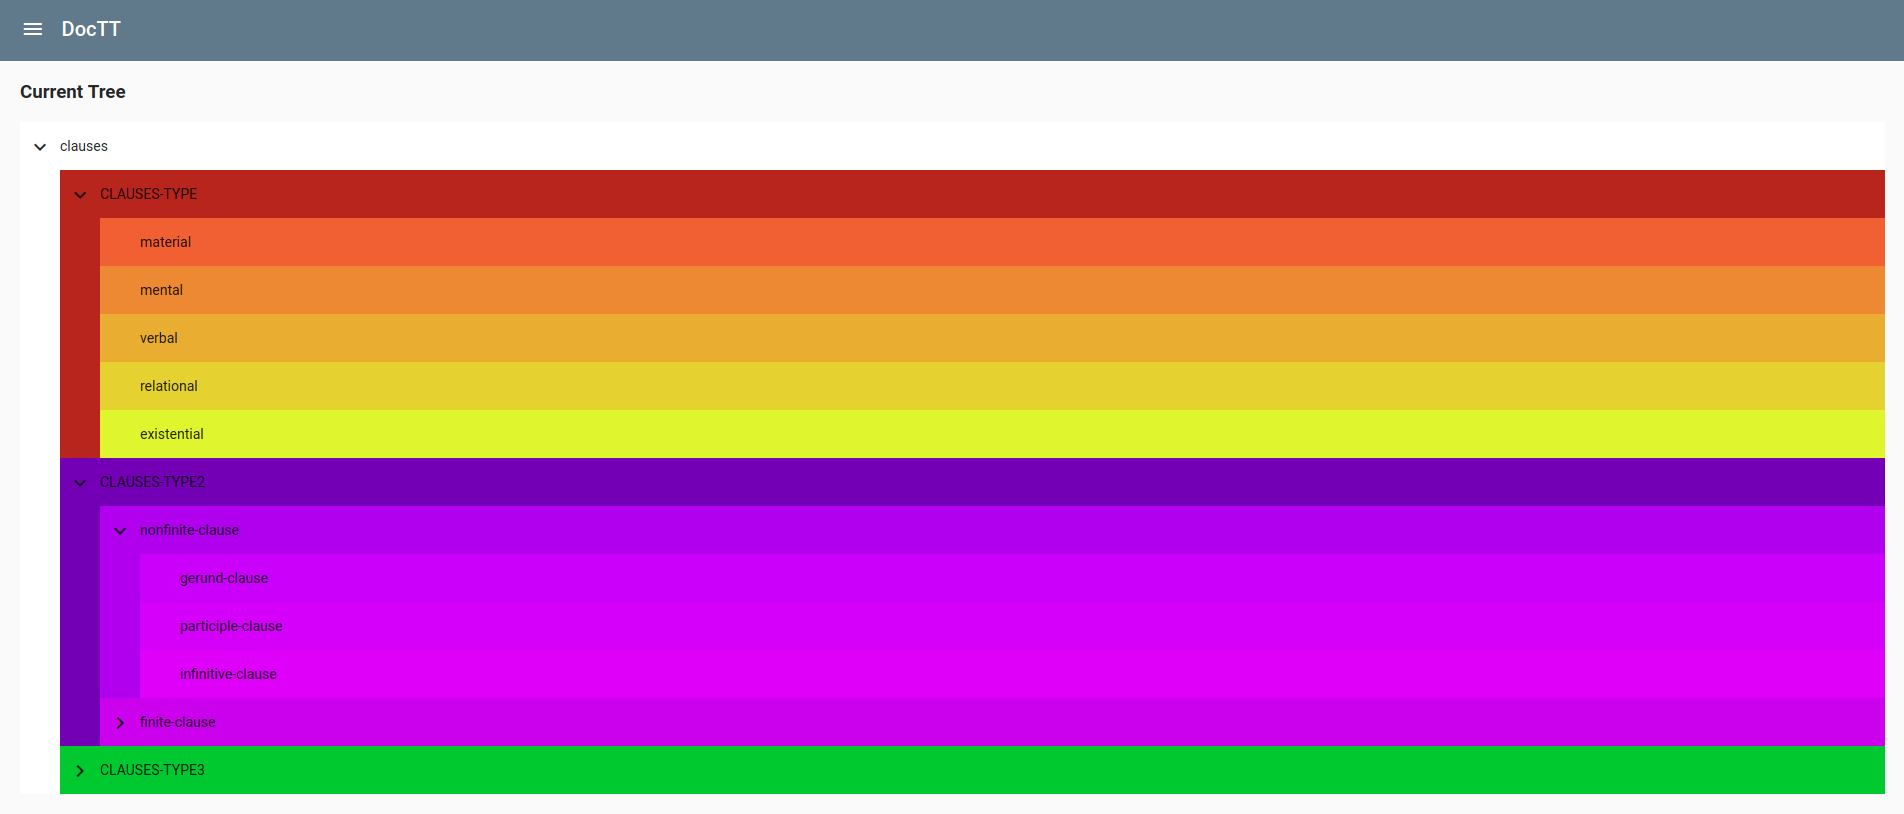
\includegraphics[width=\linewidth]{figures/treeView.png}
  \caption{Tree View section}
  \label{fig:treeView}
\end{figure}

\pagebreak

\subsection{Tree Upload}
La sezione \textbf{Tree Upload} di \textit{DocTT} è il componente che permette
l'upload dell'albero di tagging. Offre inoltre un'anteprima dell'albero 
attualmente in uso (nel caso ci fosse), secondo la stessa visualizzazione 
della sezione \textbf{Tree View}.
 
\begin{figure}[h!]
  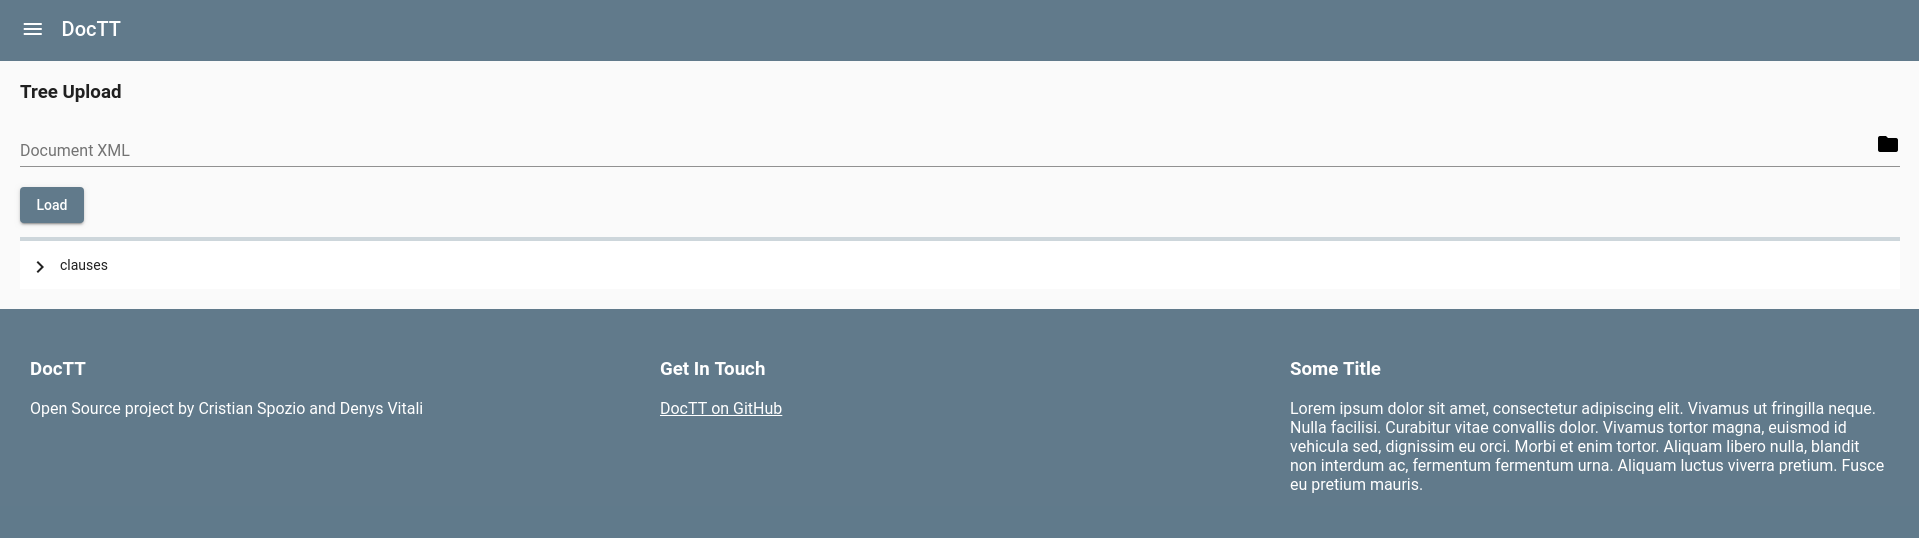
\includegraphics[width=\linewidth]{figures/treeUpload.png}
  \caption{Tree Upload section}
  \label{fig:treeUpload}
\end{figure}

\section{Tecnologie}
DocTT è stato sviluppato in \textbf{Angular}
\footnote{Angular : Framework JavaScript per la creazione di applicazioni web}
secondo le direttive fornite dal relatore. È quindi stata divisa \textit{app}
nelle sottosezioni directives, models, modules, services e shared. I 
\textit{componenti Angular} sono stati quindi divisi in 3 parti: struttura, 
stile e funzione rispettivamente secondo i linguaggi \textbf{HTML5}, 
\textbf{SCSS} e \textbf{TypeScript}.

\chapter{Funzionamento}

\section{Processo di tagging}

Il processo di tagging può venire effettuato solo dopo il caricamento di un 
albero di tagging e dopo la selezione di un documento, operazioni eseguibili
nelle apposite sezioni del tool. 

\subsection{Floating menu}

La procedura effettiva di tagging viene effettuata selezionando del testo, al
completamento di questa operazione apparirà un menu alla fine della selezione,
contenente l'albero di tagging dal quale l'utente potrà andare a scegliere
quale tag attrubuire alla selezione.

\begin{figure}[h!]
  \centering
  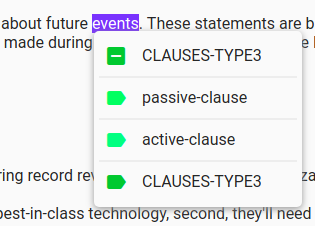
\includegraphics[width=7cm]{figures/floatingTag.png}
  \caption{Floating Tagging Menu}
  \label{fig:floatingTag}
\end{figure}

\pagebreak

\subsection{Nested tags}

Il tagging può essere effettuato a più livelli, quindi un tag (o più) possono
essere contenuti in un altro tag (o più).

\begin{figure}[h!]
  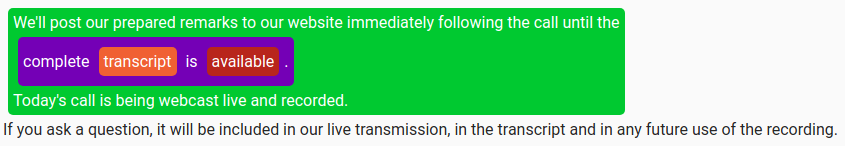
\includegraphics[width=\linewidth]{figures/nestedTags.png}
  \caption{Nested Tags Example}
  \label{fig:nestedTags}
\end{figure}

\subsection{Tag View}

Una volta taggata uan parte di testo, è possibile vedere quale tag è applicato
in quella sezione semplicemente portando il cursore sopra il suddetto tag.

\begin{figure}[h!]
  \centering
  
\includegraphics[width=7cm]{figures/sample.jpg}
  \caption{Tag View}
  \label{fig:tagView}
\end{figure}

\subsection{Tag removal}

I tag sono facilmente rimovibili semplicemente cliccando su di essi.

\begin{figure}[h!]
  \centering
  \begin{subfigure}[b]{0.4\linewidth}
    
\includegraphics[width=\linewidth]{figures/tagRemoval1.png}
    \caption{Before the click}
  \end{subfigure}
  \begin{subfigure}[b]{0.4\linewidth}
    
\includegraphics[width=\linewidth]{figures/tagRemoval2.png}
    \caption{After the click}
  \end{subfigure}
  \caption{Tag Removal Example}
  \label{fig:tagRemoval}
\end{figure}

\chapter{Specifiche tecniche}

Qui sotto verranno elencate le specifiche tecniche utilizzate durante lo
sviluppo del tool.

\section{JavaScript/TypeScript Enviroment}

Durante lo sviluppo del tool il team si è trovato a confronto con l'ambiente
di sviluppo di \textit{JavaScript/TypeScript} e quindi con le rispettive 
tecnologie, qui elencate le più significative.

\subsection{Angular}

Come già citato in precedenza, \textbf{Angular} è un \textit{web application
framework} basato su \textit{TypeScript}. Il concetto principale dietro 
\textit{Angular} è quello di definire una struttura di base ed una gerarchia
di componenti, che verranno poi inseriti all'interno del componente principale
\textit{app} come il riempimento di una cornice vuota.

\subsubsection{App structure}

Essendo \textit{app} il componente principale la sua struttura è fondamentale.
Noi abbiamo optato per suddividere il tutto, secondo convenzione di 
\textit{Angular}, in 5 parti:

\begin{description}

  \item[Directives] Le \textit{direttive Angular} sono strumenti che una volta
  definiti cambiano aspetto e/o comportamento di un elemento del DOM
  \footnote{DOM (Document Object Model): È una forma di rappresentazione di
  una pagina web come albero gerarchico}
  . 

  \item[Models] I \textit{modelli Angular} sono templates che definiscono la
  struttura di classi o interfacce.

  \item[Components] I \textit{componenti Angular} sono l'elemento base per la
  costruzione di una UI
  \footnote{UI: User Interface (Interfaccia Utente)}
  e sottostanno sempre ad una direttiva e sono spesso costruiti con dei 
  templates. Sono definiti da tre segmenti: struttura, stile e funzione.  

  \item[Services] I \textit{servizi Angular} sono dei componenti senza 
  struttura né stile, utilizzati in tutto il complesso per le loro funzioni
  e le operazioni che offrono. Possono essere visti come della classi statiche
  di utilità in \textbf{Java}.

  \item[Modules] I \textit{moduli Angular} sono una raccolta di componenti, 
  servizi, direttive, controller, filtri e informazioni sulla configurazione.
  Possono essere visti come le frazioni principali di una \textit{app}.

\end{description}

\subsubsection{Routing}

Il routing è una parte fondamentale di una qualunque applicazione front-end
che si possa definire tale. Grazie ad esso è possibile manovrare 
un’applicazione in esecuzione attraverso la richiesta di specifici path
nell’URL. Questo permette di spostarsi attraverso l'applicazione senza 
continuare a passare da una pagina web all'altra, ma semplicemente andando a
cambiare i contenuti della pagina attuale secondo le risorse richieste. Ciò 
comporta meno richieste al server ed un più rapido processo di caricamento
e \textit{switching} tra pagine/componenti.

\subsection{npm}

\textit{npm} o \textit{Node.js package manager} è un package manager per 
\textit{JavaScript}. Esso consiste in un client da CLI 
\footnote{CLI (Command Line Interface): console}
che permette all'utente di utilizzare e/o distribuire moduli 
\textit{JavaScript}.

\subsection{Webpack}

Webpack è un \textit{module bundler JavaScript} open-source. Esso permette di 
definire \textit{loaders, plugins}, ecc., utilizzato per un approccio modulare
alle \textit{web applications}.

\section{Compilazione e Test}

\subsection{Compilazione}

\subsubsection{npm}

\textit{npm} offre anche la possibilità di definire degli \textit{scripts}
utilizzabili nel suo client per utilizzi vari, nel nostro caso la compilazione.
Difatti il nostro progetto è compilabile tramite l'utilizzo del comando
\textbf{npm run build:dev} sul client \textit{npm}.

\subsection{Test}

\subsubsection{Jest}

\textit{Jest} è un framework di Testing \textit{JavaScript} basato sulla
semplicità di configurazione ed utilizzo. Permette di definire delle 
\textit{test suites}, delle collezioni di test che vadano a verificare il
corretto funzionamento e comportamento delle funzionalità del tool.

\subsubsection{npm}

Anche qui \textit{npm} si rende utile, potendo appunto definire uno
\textit{script} di testing che lancerà le varie \textit{test suites} per il
controllo tramite il comando \textbf{npm test}.

\chapter{Problemi Riscontrati}

\section{Nuovo ambiente}

Un grosso problema è stato il "nuovo ambiente" con cui ci si è dovuti 
confrontare quale il mondo di \textit{Angular}. Essendo un requisito imposto
abbiamo dovuto adattarci ed imparare il framework nel minor tempo possibile
per essere subito operativi e concentrarci sulla funzionalità del tool e le
features richieste.

\section{Comprensione differente}

All'inizio del progetto ci sono state piccole incomprensioni che hanno portato
ad un'errata implementazione, come anche lo scoprire a progetto già inoltrato
che l'albero di tagging avesse delle condizioni di tagging come restrizioni
di tipo simil-logico sul concetto di \textit{either-or} o \textit{if-then}.

\section{Mancanza di specifiche}

Essendo il tool UAM Corpus Tool (tool di riferimento dal quale dovevamo
effettuare l'integrazione) mal documentato e closed-source, abbiamo avuto
notevoli difficoltà nel capire certi tipi di scelte effettuate dagli
sviluppatori del tool. Non essendo disponibile una specifica, 
il nostro tentativo è una specie di reverse-engineering basato sull'
analisi dei file esportati mediante UAM Corpus Tool. La compatibilità
completa non è quindi garantita, specie con versioni precedenti alla 3.3.

\chapter{Piani futuri}

\section{Miglioramenti e Bug fix}

\subsection{Errore newline}

Se nella selezione compare una \textit{newline} a se stante la selezione 
riscontra problemi perché il carattere non viene rilevato come testo e quindi
non mostra il \textbf{floating menu}.

\subsection{Tag removal}

Se nel documento sono presenti per parsing errato o malformazione del documento
delle sezioni non etichettate dalla classe \textit{span-container} il 
componente non viene rilevato e quindi non viene rimosso il tag.

\section{Features}

\subsection{Tagging completo}

Come accennato nel capitolo precedente la scoperta delle restrizioni
simil-logiche hanno portato problemi durante lo sviluppo, uno dei piani futuri
è appunto quello di implementare correttamente questa feature.

\subsection{Interfaccia con IA}

Durante lo sviluppo abbiamo avuto l'occasione di relazionarci con un 
masterando partecipante al progetto che stava lavorando su una rete neurale
capace di effettuare il tagging in automatico dei documenti. Un'aggiunta
possibile sarebbe quella di interfacciare il tool con il lavoro del masterando
e quindi al momento dell'upload di un documento effettuare questo tagging
automatico iniziale sul quale poi l'utente andrà a lavorare.

%Citazione:
%\begin{quote}
%\lipsum[23]
%\end{quote}

%\lipsum[13]

%\begin{itemize}
%  \item Elemento A
%  \item Elemento B
%  \item Elemento C
%\end{itemize}

%\begin{itemize}
%  \item[-] Elemento A
%  \item[-] Elemento B
%  \item[-] Elemento C
%\end{itemize}
%
%\begin{enumerate}
%  \item Alpha
%  \item Beta
%  \item Gamma
%\end{enumerate}

%\lipsum[23]
%\section{Sezione}
%
%\lipsum[23]
%
%\subsection{Sotto sezione}
%
%Un po' di matematica: \newline
%
%\begin{math}
%\frac{n!}{k!(n-k)!} = {n \choose k}
%\end{math} \newline
%
%Un po' di matematica centrata:
%
%\begin{center}
%\begin{math}
%\frac{n!}{k!(n-k)!} = {n \choose k}
%\end{math}
%\end{center}
%
%Oppure con \$\$
%
%$$
%\frac{n!}{k!(n-k)!} = {n \choose k}
%$$
%
%Oppure anche direttamente nel testo ${1}\over{n}$ \\
%
%\lipsum[23]

\bibliographystyle{unsrt}
\bibliography{bibliografia}
\end{document}
